\chapter{AbaaS - Atomic Broadcast as a Service}

% **************************** Define Graphics Path **************************
\ifpdf
    \graphicspath{{Chapter3-TxService/Figs/Raster/}{Chapter3-TxService/Figs/PDF/}{Chapter3-TxService/Figs/}}
\else
    \graphicspath{{Chapter3-TxService/Figs/Vector/}{Chapter3-TxService/Figs/}}
\fi

%Introduction

This chapter introduces the concept of providing \emph{abcast} messaging as a service to members of a cluster.

First we describe the rational behind \textsf{Abaas}, then we explore the requirements of such a service and the challenges involves in meeting them.  This is followed by the introduction of the \textsf{ABService} protocol that is used to implement \textsf{AbaaS}.  We then explain the methodology used to evaluate \textsf{ABService}, before presenting the results of our performance evaluation.  Finally, we discuss the limitations of existing \emph{abcast} protocols in the context of \textsf{AbaaS}, and propose the need for a new non-blocking \emph{abcast} solution.  

\section{Rational}
Total order commit protocols can be utilised by distributed systems to coordinate transactions without the use of locks.  Reducing the abort rate of transactions when contention is high, as system deadlocks do not occur when distributed locks are not present.  Therefore, total order commit protocols can aid scalability as they improve transaction throughput \citep{Ruivo:2011:ETO:2120967.2121604}.  

The limiting factor of total order commit protocols is the underlying \emph{abcast} protocol used to provide atomic guarantees on message delivery.  The TOA protocol currently utilised by Infinispan, does not scale well as the number of destinations $N$ increase, as $N->1$ communication is expensive ($\S$ \ref{ssec:TOA_limations}).  Similarly, other GM protocols such as Newtop \citep{Ezhilchelvan:1995:NFG:876885.880005}, exasperate the problem, as the number of messages required to perform an \emph{abcast} increases dramatically as $N$ increases.  Finally, Quorum based protocols provide even less scalability, then GM based protocols, as their inability to \emph{abcast} messages to disjoint sets of nodes typically requires all nodes in the cluster to participate in an \emph{abcast}.  

Regardless of the \emph{abcast} protocol used, $N->1$ communication is inherently unscalable.  Therefore, we propose that reaching a consensus on \emph{abcast} ordering should not be conducted between a transaction coordinator $Tx.c$ and its participating Infinispan nodes $Tx.dst$, but instead atomic ordering should be provided by an independent coordination service and consumed by $Tx.c$.  It is then the responsibility of $Tx.c$ to coordinate $Tx$, with $Tx.dst$, using the ordering provided by this service.  We call this system model Atomic Broadcast as a Service (\textsf{AbaaS}), and refer to the existing Infinispan approach as \emph{peer-to-peer} (P2P).  

Utilising \textsf{AbaaS} decouples message broadcasting and message ordering, by restricting the number of nodes conducting \emph{abcast} messages to the nodes providing the service; known as \emph{service} nodes, or simply $s$-nodes, and denoted as $N_s$; Infinispan nodes are known as \emph{client} nodes, or simply $c$-nodes, and denoted as $N_c$.  This decoupling means that regardless of $\left\vert Tx.dst \right\vert$, the number of nodes that execute a \emph{abcast} protocol, to obtain a total order for $Tx$, will always be equal to $\left\vert s\text{-nodes}\right\vert$.  Furthermore, restricting \emph{abcast}s to $s$-nodes means that, for all \emph{abcast}s, $m.dst$ will be the same, therefore \emph{abcast}s always occur between a single destination set, which increases performance ($\S$ \ref{ssec:single_destination_set}) and enables certain optimisations to be made ($\S$ \ref{ssec:abaas_optimisations}).  

	Lastly, implementing transaction ordering as a dedicated service, provides distinct advantages for system administrators.  When utilising the P2P \emph{abcast} approach, administrators would typically want to run Infinispan over a cluster of nodes utilising a homogeneous hardware specification to ensure that Infinispan's performance would not be hindered by a lesser machine.  In an environment where low-latency and high-capacity in-memory database is desired, this would require a large number of expensive machines. However, when AbaaS is utilised, it is possible to improve the performance of the entire cluster, simply by upgrading the $s$-nodes used to provide the \emph{AbaaS} service.  For example, consider a cluster consisting of $50$ $c$-nodes, and $3$ $s$-nodes, instead of upgrading all $50$ $c$-nodes it is possible to improve transaction latency and throughput by upgrading the hardware of the $3$ $s$-nodes.  
	
	\subsection{Optimisations}\label{ssec:abaas_optimisations}
	The \textsf{Abaas} model allows for two key optimisations that are not possible when \emph{abcast}ing occurs directly between $N_c$ nodes: \emph{Message Bundling} and \emph{Acknowledgement Piggybacking}.  
	
		\subsubsection{Message Bundling} \label{ssec:bundling} \hspace{0pt} \\
		As the number of concurrent transactions between $c$-nodes increases, the total number of \emph{abcast}s required also increases.  When utilising \emph{abcast}s between $c$-nodes to coordinate the transactions, typically it is not possible to bundle multiple \emph{abcast} messages $<m_i, m_j>$, into a single \emph{abcast}, $m$, due to the high probability of $m_i.dst \neq m_j.dst$.  Of course it is possible to implement a bundling strategy that is utilised only when $m_i.dst = m_j.dst$, however in a system such as Infinispan the performance improvements provided by such a strategy are negligible; as the wide distribution of key/value pairs significantly reduces the probability of two \emph{abcast}s having the same destination set.  
		
		However, when utilising \textsf{AbaaS} it is possible for all \emph{abcast} requests received from $c$-nodes to be bundled at a receiving $s$-node, regardless of their destination set.  This is because $s$-nodes only send \emph{abcast}s to other $s$-nodes, therefore the destination set is the same for all $c$-node requests.  
		
		The ability to bundle multiple \emph{abcast} requests into a single \emph{abcast} reduces the number of times that a consensus needs to be reached between all $s$-nodes.  This further reduces the number of $N->1$ communication steps required, with the total number of \emph{abcast}s reduced by $\left\vert bundle \right\vert$; where $bundle$ is the amount of \emph{abcast} requests sent as a single \emph{abcast}.  Therefore, significantly reducing the total amount of network traffic when requests are frequent, resulting in the capacity and scalability of an \emph{AbaaS} service increasing.  Furthermore, message bundling does not compromise performance when the number of service requests is low, as bundling does not require any additional communication steps or intensive computation.  
		
		\subsubsection{Acknowledgement Piggybacking} \hspace{0pt} \\
		As all $s$-nodes send \emph{abcast}s to all other $s$-nodes, and hence, always have the same destination set, it is possible for message acknowledgements to be piggybacked, therefore enabling \emph{abcast}s to be completed with just a single dedicated broadcast ($\S$ \ref{ssec:newtop}).  This optimisation is ideal for a \textsf{AbaaS} service: as all nodes in the service must handle $c$-node requests, thus ensuring that each $s$-node frequently sends \emph{abcast}s containing piggybacked acknowledgements; and, it aids scalability as it reduces the number of messages sent over the network. 	
	
\section{Limitations of Existing Coordination Services}\label{sec:limitations_existing_coordination}
It is possible to utilise existing coordination solutions ($\S$ \ref{sec:coordination}), such as Zookeeper\citep{Hunt:2010:ZWC:1855840.1855851} and Chubby\citep{Burrows:2006:CLS:1298455.1298487}, as a basis of a \textsf{AbaaS} service.  However, both of these solutions are intended for high levels of read requests, not workloads that consist predominantly of write operations; an operation that changes the state of a single service node requires all other service nodes to update their state (i.e. a client ordering request), and is classified as a write operation.  

Write requests are vital to the \textsf{AbaaS} model, as every client request needs to be forwarded to all $s$-nodes within a service to ensure consistency (S1, S2).  Both of these existing services rely on a establishing a quorum amongst $s$-nodes for each write operation, which is coordinated by a single master node, and as a result, performance deteriorates rapidly as the number of write requests increase.  Therefore, if Zookeeper or Chubby were utilised as the basis of a \textsf{AbaaS} service, the service's latency and throughput would be poor as neither solution is intended for write-dominated workloads.  The observed limitations of these existing solutions is the motivation for requirement S3 in $\S$ \ref{sec:absaas_requirements}.  	
	
\section{System Requirements}\label{sec:absaas_requirements}
The \textsf{AbaaS} model consists of two distinct entities: $s$-nodes and $c$-nodes.  This section will explore the requirements that need to be met in order for the \textsf{AbaaS} model to be effective.  We consider requirements from the perspective of both clients, $c$-nodes, and the ordering service, $s$-nodes.

	\paragraph{Client Requirements} \hspace{0pt}
	\begin{itemize}
		\item [\textbf{CR1}] Clients must be able to send \emph{abcast}s to multiple destination sets that may overlap.
		
		\item [\textbf{CR2}] The service must provide a consistent total order $m.ts$ on messages irrespective of the $s$-node handling a clients request, or the $c$-node from which the clients request originated.  
		
		\item [\textbf{CR3}] Client nodes must be informed of $m_i$ when handling $m_j$, if $m_i.dst \cap m_j.dst$ to ensure that $m_i$ is not missed by a $c$-node in $m_i.dst$.  
	\end{itemize}
	
	\paragraph{Service Requirements} \hspace{0pt}
	\begin{itemize}
		\item [\textbf{S1}] The service must provide fault-tolerance ($s\text{-nodes} > 1$).
		
		\item [\textbf{S2}] The service must be highly available and non-blocking in the event of $s$-node failures.  Necessary to prevent the entire cluster becoming blocked if a $s$-node fails.   
		
		\item [\textbf{S3}] All service nodes must process client requests in the exact same order to maintain a consistent state between all $s$-nodes.  This prevents a $c$-node from receiving conflicting ordering data, for example two distinct $m$ being allocated the same global timestamp.  
		
		\item [\textbf{S4}] All $s$-nodes should be able to handle client requests, to allow for high availability and to prevent a single $s$-node becoming a performance bottleneck.
	\end{itemize}

\section{Protocol Details}\label{sec:decoupled_protocol}
% Change protocol name from Dcup
We have developed a protocol for the \textsf{AbaaS} model, which we call \textsf{Dcup}; as from the $c$-nodes perspective it decouples \emph{abcast} ordering and broadcast.  \textsf{Dcup} satisfies all of the requirements specified in $\S$ \ref{sec:absaas_requirements} with the exception of S2.  S2 cannot be satisfied by our protocol directly, rather \textsf{Dcup} relies on a \emph{abcast} protocol to guarantee S1, S3 and S4, therefore in order for S2 to be satisfied, the underlying \emph{abcast} protocol must not block in the presence of node failures.  

\textsf{Dcup} consists of six distinct phases, each of which are explored below.  In the explanation below we assume that Infinispan is executing a 1-Phase Total Order transaction, without a second WSC phase, and that the transaction has already been successfully executed locally.  Furthermore, we assume that a reliable network protocol is being utilised as the underlying communication mechanism, for example TCP\citep{Cerf:2005:PPN:1064413.1064423} or Reliable UDP\citep{ReliableUDP}.  Finally, we refer to a collection of $s$-nodes providing \emph{abcast} ordering as the \emph{ordering service}.  

	\begin{description}
		\item[1. Client Request - Client] \hfill \\
		Once a $Tx_i.c$ has completed its local execution of $Tx_i$, it is ready to \emph{abcast} a $prepare(Tx_i)$ message to $Tx_i.dst$ as required by the total order commit protocol.  In \textsf{Dcup} \emph{abcasts} are initiated by the $Tx_i.c$ randomly selecting a $s$-node, $N_s$, from the \emph{ordering service}, and sending an \emph{abcast} request $r(Tx_i)$ to $N_s$.  
		
		The content of the $prepare(Tx_i)$ message is not sent to $N_s$ as we only require a global order for $Tx_i$, therefore the contents of the message to be \emph{abcast} is irrelevant and including it would only increase the load on the network.  However, all order requests must specify $Tx_i.dst$ as this is the destination set of the \emph{abcast} that $Tx_i$ is trying to send, and the \emph{ordering service} needs this data to ensure that requirements CR1, CR2 and CR3 are satisfied.  
		
		\item[2. Receive Request - Ordering Service] \hfill \\
		Upon receiving $r(Tx_i)$, $N_s$ places the request in the \emph{Abcast Request Pool} (ARP), which is a bounded queue used for storing requests before they are processed by an $s$-node.  If an $s$-node's ARP becomes full, subsequent requests from $c$-nodes are rejected until space becomes available in the ARP.  When a $c$-node request is rejected a \emph{reject} response is sent to $Tx_i.c$ whom can then abort $Tx_i$ or resend $r(Tx_i)$ after a configurable amount of time.    
		
		The ARP is necessary to ensure that if the \emph{ordering service} starts to become overloaded by client requests their is a 'feedback' mechanism that makes clients aware of the services current limitations, allowing clients to restrict user operations if necessary.  Utilising an ARP is also essential for providing message bundling, which as described in \ref{ssec:bundling} is an effective optimisation for improving the throughput of an \emph{ordering service}.  
		
		\item[3. Process ARP - Ordering Service] \hfill \\
		A single thread, called the \emph{send} thread, is utilised for retrieving requests from the ARP and \emph{abcast}ing them to all $s$-nodes for ordering.  If the ARP is empty, then the \emph{send} thread waits for the ARP to become non-empty before resuming \emph{abcast}ing.  The \emph{send} thread retrieves ordering requests from the ARP in their arrival order, and bundles them into a single message bundle $mb$, before \emph{abcast}ing $mb$ to all $s$-nodes.  
		
		A configurable upper limit is placed on the maximum size (number of messages or \emph{bytes}) of a bundle message.  If this upper limit is reached and the ARP still has available requests, then the \emph{send} thread will \emph{abcast} the next message bundle $mb'$ once $mb$ has been \emph{abcast}.  If message bundling is not enabled, then a upper limit of one message is set for all $mb$.  
		
		All \emph{abcast} $mb$, that are sent by $N_s$ have their originator set to $N_s$, $mb.o$ = $N_s$.  This is necessary for the next phase of the protocol.  
		
		\item[4. Receive Ordering - Ordering Service] \hfill \\
		When a $s$-node, $N_s$, receives an request bundle $mb$, it 'un-bundles' $mb$ and processes each ordering request $r(Tx)$ in the order that they arrived in the ARP at $mb.o$.  Each $r(Tx)$ is then assigned a global timestamp $ts$: $r(Tx_i).ts = m.ts\oplus m.o \oplus$\emph{sequence number} of $r(Tx_i)$ within the bundle; where $\oplus$ is the append operator and $m.ts$ is the final timestamp provided by the underlying \emph{abcast} protocol utilised between $s$-nodes.  If $N_s = mb.o$, then $N_s$ is the $s$-node that initially received $r(Tx_i)$, therefore $N_s$ must send a response message to $Tx_i.c$.    
		
		A Response message consists of two types of ordering data: $ts$ agreed by $s$-nodes for $r(Tx_i)$, and $r(Tx_i)$'s \emph{immediate} predecessor.  The latter is the identity of $r(Tx_j)$ whose delivery at the specified $c$-node must \emph{precede} \emph{immediately} before delivery of $r(Tx_i)$.  More precisely, $d \in r(Tx_i).dst$, $d$ must not deliver $r(Tx_i)$ until it delivers $r(Tx_j)$, and no \emph{abcast} other than $r(Tx_i)$ must be delivered immediately after $r(Tx_j)$ is delivered.
		
		The storage of \emph{immediate} predecessor data works as follows: All $s$-nodes maintain a map that stores a transaction history by mapping a $c$-node address with the id of the last transaction they were associated with, hence its \emph{immediate} predecessor.  So for each $r(Tx)$ the associated $r(Tx).ts$ is stored in the map for each $d \in Tx.dst$. When a $s$-node receives an \emph{abcast} bundle $mb$, it knows that all other $s$-nodes have received, or will receive, $mb$ in the same order.  Therefore, when $mb$ is processed by an $s$-node, as it is guaranteed that all other $s$-nodes will have processed $mb$ in the exact same order, we know that the transaction history will be consistent at all $s$-nodes.  
		
		Note that the immediate predecessor of $r(Tx_i)$ is applicable to \emph{all} \emph{abcast}s directed at a given $d$ - not just those that originate from $Tx_i.c$ nor just those that are handled only by $N_s$. Thus, it is specific to each $d$ and ensures that delivery at every $d$ is as per the finalized $r(Tx).ts$. To illustrate this, let $Tx_i.c$ submit $r(Tx_i)$ to $N_s$, $Tx_j.c$ submit $r(Tx_j)$ to $N_{s'}$ and $d \in Tx_i.dst \cap Tx_j.dst$. Say, $s$-nodes order $r(Tx_j)$ before $r(Tx_i)$. If $d$ receives $r(Tx_i)$ before $r(Tx_j)$, it will not deliver $r(Tx_i)$ until it delivers $r(Tx_j)$.

    \item[5. Receive Ordering Response - Client] \hfill \\
    When $Tx_i.c$ receives $r(Tx_i)$ from $N_s$, it appends the original $prepare(Tx_i)$ message to $r(Tx_i)$ and broadcasts it to all $Tx.dst$, before executing $prepare(Tx_i)$ locally.  
    
    \item[6. Receive Broadcast - Client] \hfill \\
    Upon receiving $r(Tx_i)$, a $c$-node, $c$, will check the \emph{immediate} predecessor data that is applicable to $c$, $r(Tx_j)$.  If $r(Tx_j)$ has been received by $c$ then $r(Tx_i)$ can be delivered by $c$ and the $prepare(Tx_i)$ operation is executed.  However, if $r(Tx_j)$ has not yet been received by $c$ then $r(Tx_i)$ cannot be delivered locally, and $c$ must wait to receive $r(Tx_j)$ before delivering $r(Tx_i)$.  
    
    A single $ts$ is provided for each $d \in Tx.dst$ in the predecessor data, opposed to a list of past timestamps for each $d$, in order to reduce the size of each $r(Tx)$.  This results in a cascading wait occurring if multiple messages have not yet been received by $c$.  For example, if $c$ has received $r(Tx_i)$ but has not received its predecessors $r(Tx_j)$ and $r(Tx_k)$, $c$ is only aware of $m.j$, however when $r(Tx_j)$ arrives, it reads $r(Tx_j)$'s predecessor data and becomes aware that it has not yet received $r(Tx_k)$ and must therefore wait for $r(Tx_k)$ before delivering $r(Tx_j)$ and $r(Tx_i)$.  
    
   	\end{description}

	\subsection{Fault-Tolerance}
	Fault-tolerance in \textsf{Dcup} must consider the consequences of both crashed $c$-nodes and $s$-nodes.  Here we explore the consequences of $c$-node, and then $s$-node crashes during various stages of a \textsf{Dcup} \emph{abcast} and how they are mitigated.  In this section we consider node crashes from the perspective of a single transaction, however it is worth noting that each $c$-nodes would typically have multiple transactions executing concurrently.  
	
	\paragraph{Client Node Crash} \hspace{0pt} \\
	When a $c$-node, $c$, crashes during or directly after the local execution of $Tx_j$ then no action needs to be taken for this $Tx$, as no interactions with other nodes has occurred.  
	
	If $c$ crashes between steps 1 and 5 of \textsf{Dcup}, then no $c$-nodes will receive the transaction message $r(Tx_j)$ as $c$ is unable to broadcast $r(Tx_j)$ to all $Tx_i.dst$.  As a consequence, the transaction history recorded by the \emph{ordering service} will be inconsistent with the actual messages broadcast by $c$; meaning that all $d \in Tx.dst$ will expect to receive $r(Tx_j)$ from $c$ because the predecessor information in subsequent messages $r(Tx_i)$ state that $r(Tx_j)$ is required.  Such a scenario would lead to deadlock occurring for all $d \in Tx.dst$, as $r(Tx_j)$ will never arrive.  
	
	To prevent deadlock from occurring, in the event of a $c$-node crashing, the ordering service will broadcast a $CRASH_AWARE$ message to all $c$-nodes who have recently participated in transactions with $c$; where recent participation can be defined temporally or based upon the number transactions that have subsequently been executed.  A $CRASH_AWARE$ message consists of the last $x$ responses sent by the \emph{ordering service} to $c$.  When a $c$-node $c'$ receives the $CRASH_AWARE$ message, it becomes aware of $c$'s recent message history, and therefore it can ignore any message $r(Tx_j)$ that originated at $c$ that has not been received, whilst also becoming aware of $r(Tx_j)$ predecessor as specified in $r(Tx_j)$. Thus deadlock is prevented, but $c'$ knows to wait for any missing predecessor messages.  
	
	Ideally $x$ should be equal to the maximum number of concurrent transactions that can executed on a given $c$-node as this is the maximum number of transactions, $\#Tx$, that could have been executing when $c$ crashed, therefore this is the maximum number of messages that could have been missed during a single $c$-node failure.  In order for the service to be tolerant of $n$ $c$-node failures, $x$ needs to be defined as follows: $x = n\#Tx$.  
	    
	\paragraph{Service Node Crash} \hspace{0pt} \\
	If a $s$-node $N_s$ crashes before stage 3 of \textsf{Dcup}, then the $Tx.c$ that requested a message ordering from $N_s$ will not receive an ordering response.  Instead, $Tx.c$ will eventually timeout, at which point $Tx.c$ can either resend the request to a different $s$-node, or abort the transaction.  As this scenario only involves $N_s$, and no other $s$-node, a timestamp is not assigned to $Tx$ and so it is not possible for deadlock to occur.  
	
	If a $s$-node, $N_s$, crashes during stages 3 or 4 of the \textsf{Dcup} protocol, after receiving $r(Tx_i)$ from $Tx_i.c$ and \emph{abcast}ing $r(Tx_i)$ it to all $s$-nodes, it is possible for all operative $s$-nodes to receive $r(Tx_i)$ before $N_s$ crashes.  But because $N_s$ has crashed, it is not possible for $N_s$ to send $r(Tx_i)$ to $Tx_i.c$.  This means that the record maintained by the still operative $s$-nodes will state that $Tx_i$ has ordering $r(Tx_i).ts$, however $Tx_i.c$ will never be able to broadcast $r(Tx_i)$ to $Tx_i.dst$ as it never received a response from $N_s$ and consequently all $d \in Tx_i.dst$ will be in a state of deadlock as they wait indefinitely for $r(Tx_i)$.  
	
	To prevent deadlock, a $CRASH_AWARE$ message is sent by a/all remaining $s$-node(s) to the $Tx.c$ of \emph{all} $c$-nodes involved in the last $x$ responses sent by the \emph{ordering service}.  Upon receiving the $CRASH_AWARE$ message, any $Tx.c$ waiting for a response header will have received its ordering, albeit in a atypical manner and can now execute stage 6 of \textsf{Dcup}.  
	
\section{Experimentation}
% Explain - 10 clients, x box members etc.  Utilise Aramis paper
% Flow control used in the box and in traditional TOA.  

To test our assumption that the \textsf{AbaaS} model would improve transaction performance, we developed an experiment that utilises the \textsf{AbaaS} Protocol (\ref{sec:decoupled_protocol}).  The details of these experiments are outlined below. 

\paragraph{AbaaS Experiment} \hspace{0pt} \\
We implemented an \textsf{AbaaS} service using the JGroups\citep{JGroups} framework with $n=2$ and $3$ $s$-nodes.  All nodes in the experiment utilised commodity PCs of \emph{2.80GHz Intel Core i7} CPU and 4GB of RAM, running \emph{Fedora 19} and communicating over Gigabit Ethernet. The $s$-nodes are a part of a large university cluster, hence communication delays between them can be quite volatile as they are influenced by other network traffic and by jobs launched on $s$-nodes by other users.

Our experiments are based upon a highly modified version of an existing performance test available in the JGroups\citep{JGroups} framework, that mimics the partial replication of key/values in Infinispan\citep{Infinispan}.  In these experiments we utilise ten $c$-nodes in the same cluster, each of which emulates a transaction system that is reliant on the \textsf{AbaaS} service.  Each $c$-node operates 25 concurrent threads to initiate and coordinate transactions, and a transaction $Tx$ involves a set $Tx.dst$ of $3,4,\ldots,10$ $c$ nodes (including its coordinator). Each $Tx$ consists purely of key/value write operations and hence requires \emph{abcast} for completion. Read requests ($get(k)$) are not emulated, as the retrieval of key/values occurs before $Tx.c$ \emph{abcast}s its $prepare(k)$ message, and therefore has not baring on \emph{abcast} performance.  A thread coordinating a transaction starts the next $Tx'$ as soon as it dispatches commit/abort decision for the current $Tx$. Thus, at any moment, $250$ transactions are in different stages of execution.

A coordinator thread submits its \emph{abcast} request for $Tx$, denoted as $r(Tx)$, with some $s$-node; the latter stores such requests in the ARP in the arrival order. The \emph{Send} thread bundles some or all of these requests in the ARP in their arrival order into a message bundle $mb$, which can have a maximum payload of $1kB$, then \emph{abcast}s $mb$ to all other $s$-nodes.  The \emph{Send} thread waits if the ARP is empty and resumes bundling once ARP becomes non-empty. Thus, the number of requests bundled in any $mb$ varies depending on the request arrival rate. Once $r(Tx)$ has been \emph{abcast} to all $s$-nodes, it is returned to $Tx.c$ whom disseminates the message to $Tx.d$.  When all $d \in Tx.dst$ have received $r(Tx)$, the transaction is considered complete and the coordinator thread can start executing $Tx'$.  

\paragraph{P2P Experiment} \hspace{0pt} \\
In order to test the performance of P2P total order commits we repeated the  experiments detailed above, however $c$-nodes coordinate transactions between themselves without utilising any $s$-nodes.  Furthermore, the same cluster, and commodity machines were used for all experiments to ensure a fair comparison.   

\section{Performance Evaluation and Comparison}\label{sec:abaas_results}
Performance evaluation focuses on the comparison of a \textsf{Base} protocol (TOA), being utilised in a traditional P2P scenario (\emph{BaseP2P}), with an \textsf{AbaaS} service that implements the \textsf{Dcup} protocol and utilises the same \textsf{Base} protocol between $s$-nodes (\emph{BaseService}).

Our performance comparison focuses on comparing transaction latency and throughput between \emph{BaseP2P} and \emph{BaseService}.  In \emph{BaseService}, latency is measured as the time elapsed between a $c$-node's initial transmission of $r(Tx)$ to some $s$-node, and all members of $Tx.dst$ delivering $r(Tx)$ to the experiment application. In BaseP2P, latency is measured as the time taken for all $Tx.dst$ to deliver $Tx$ to the experiment application. For both approaches, throughput is measured as the average number of \emph{abcast}s delivered by the experiment application per second at each $c$-node.

All of our experiments were conducted in isolation in order to prevent any side effects caused by simultaneous execution across the cluster, however we conducted all experiments during the same time period to ensure that the network was under similar loads for all of our experiments. 

\begin{figure}[htbp!]
 % \centering
 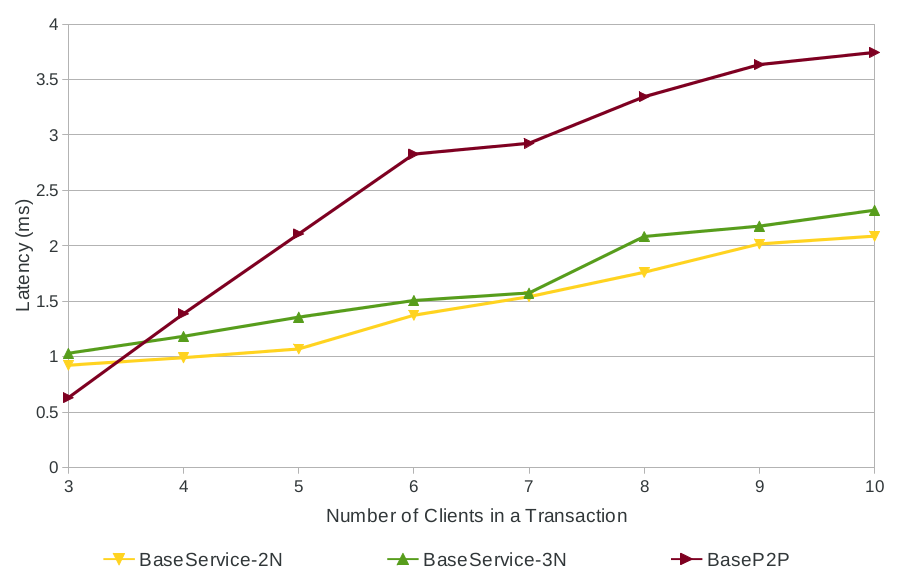
\includegraphics[width=\textwidth,height=\textheight,keepaspectratio]{latency}
 \caption{Comparison of Latency}
 \label{fig:LatencyGraph}
\end{figure}

\begin{figure}[htbp!]
% \centering
 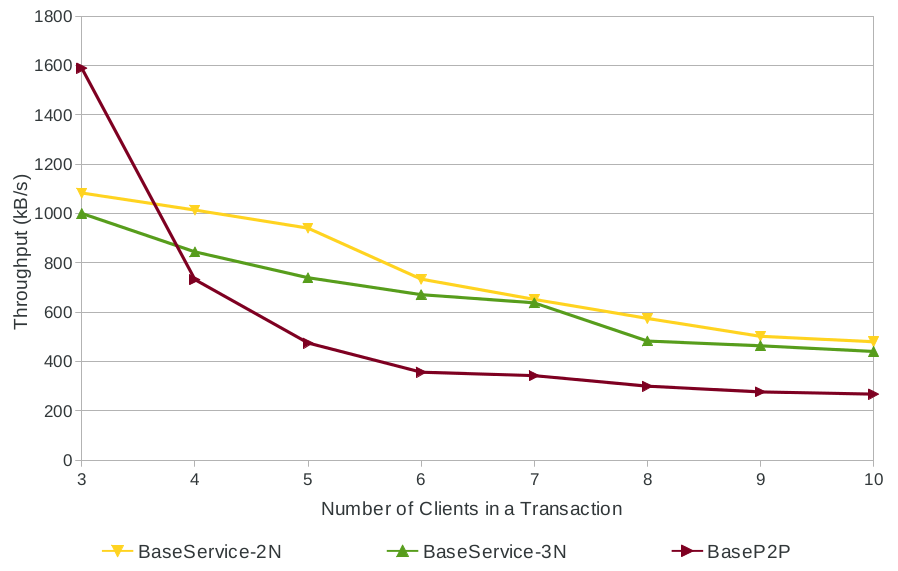
\includegraphics[width=\textwidth,height=\textheight,keepaspectratio]{throughput}
 \caption{Comparison of Throughput}
 \label{fig:ThroughputGraph}
\end{figure}

Figures \ref{fig:LatencyGraph} and \ref{fig:ThroughputGraph} show latency and throughput, with $2N$ and $3N$ representing an \emph{ordering service} that consists of two and three, $s$-nodes respectively.  Each plot on the graph is an average of three \emph{crash-free} trials; a trial consists of each $c$ node completing $10^4$ transactions for a specific value of $|Tx.dst|$. Thus, BaseService receives a total of $10^5$ \emph{abcast} requests in each trial. In BaseP2P, each $c$ node initiates $10^4$ Base executions with its peers and the steady throughput in Figure \ref{fig:ThroughputGraph} as $|Tx.dst| \rightarrow 10$ suggests an absence of node saturation.

Referring to Figure \ref{fig:LatencyGraph}, as $|Tx.dst| \geq 4$, BaseP2P's \emph{abcast} latencies increase considerably, indicating that \emph{abcast}ing is best provided as a service for scalable performance. Comparing throughput in Figure \ref{fig:ThroughputGraph} leads to similar conclusions.  

BaseP2P's superior performance when $Tx.dst < 4$ can be attributed to the additional stages involved when utilising the \emph{AbaaS} model.  For example when BaseService utilises two $s$-nodes ($2N$) the following stages are required: $Tx.c$ sends a request, the \emph{ordering service} \emph{abcast}s it with $|m.dst| = 2$ and returns it to $Tx.c$, who must then broadcast $r(Tx)$ to $Tx.dst$.  Ignoring the individual message cost of each stage the total number of stages is four, whereas in BaseP2P the only step required is the \emph{abcast}ing of $Tx$.  So although $|m.dst|$ for each \emph{abcast} is less in BaseService ($|m.dst| = 2$) than BaseP2P ($|m.dst| = 3$), the overhead of sending a request to the \emph{ordering service} and back is much greater than the savings offered by reducing $|m.dst|$ by one node.  However, as $|Tx.dst|$ increases, the overhead of BaseP2P's increased $|m.dst|$ becomes significant, to the point where BaseService's additional communication stages becomes less of an overhead than the cost BaseP2P \emph{abcat}ing to a large $m.dst$.  

\paragraph{Summary} \hspace{0pt} \\
When deploying a large-scale distributed transaction system, higher throughout and lower-latency can be achieved by utilising a separate service to provide \emph{abcast} capabilities when the the number of nodes participating in a transaction is greater than three.  

\section{A New Atomic Broadcast Solution is Required}
Section \ref{sec:abaas_results} clearly shows that transaction throughput can be improved by utilising the \textsf{AbaaS} model for \emph{abcast} ordering.  However, the existing protocol used, TOA, is a GM based protocol that blocks severely when node crashes occur.  This blocking behaviour is acceptable when TOA is utilised between client nodes, as it is presumed that blocking will only occur at a small subset of the overall cluster, thus system \emph{liveness} still exists in the majority of the cluster.  However, if all $s$-nodes utilise TOA for \emph{abcast}ing and a single $s$-node crashes, all $s$-nodes will block, resulting in no client requests being satisfied. Therefore, not only are the $s$-nodes blocked, but as a consequence of this blocking, so is the entire cluster.  Thus the entire system's \emph{liveness} is lost until the GM protocol detects the $s$-node crash and unblocks the ordering service.  GM based protocols, such as TOA, cannot be used as the basis of a \textsf{AbaaS} service as system-wide blocking would be catastrophic for any in-memory database.  

As detailed in sections \ref{sec:limitations_existing_coordination} and \ref{sec:coordination}, quorum based \emph{abcast} protocols are not suitable for use in \textsf{AbaaS} due to their tendency to block mildly when the master is falsely/validly suspected of crashing, and because of the performance limitations associated with master based protocols.  

Therefore, in order for \textsf{AbaaS} to be valid system model, a new \emph{abcast} protocol is required.  The \emph{abcast} protocol must allow for low-latency, high-throughput \emph{abcast}s, as provided by GM based protocols, in addition to providing non-blocking behaviour in the presence of node failures.  

\section{Summary}
This chapter presents a new model for \emph{abcast} protocols that decouples message ordering and sending.  We present a new protocol \textsf{Dcup} for use in such an environment, and detail an experiment that allows for the performance of \textsf{AbaaS} and P2P protocols to be evaluated.  Performance evaluation shows that \textsf{AbaaS} provides superior performance over the existing P2P approach as the number of nodes in a transaction increases.  Finally, we outline the need for a new \emph{abcast} protocol for use within an \textsf{AbaaS} service. 